\documentclass[10pt,t]{beamer}
\usetheme{Madrid}
\setbeamercovered{transparent}

% ── Course colour palette (teal matches course branding) ──────
\definecolor{CourseTeal}{RGB}{0,178,189}
\definecolor{CourseDark}{RGB}{18,32,58}
\definecolor{CourseGrey}{RGB}{240,247,249}

\setbeamercolor{palette primary}{bg=CourseDark,fg=white}
\setbeamercolor{palette secondary}{bg=CourseTeal,fg=white}
\setbeamercolor{palette tertiary}{bg=CourseTeal!55!CourseDark,fg=white}
\setbeamercolor{palette quaternary}{bg=CourseDark,fg=white}
\setbeamercolor{structure}{fg=CourseTeal}
\setbeamercolor{frametitle}{bg=CourseDark,fg=white}
\setbeamercolor{title}{bg=CourseDark,fg=white}
\setbeamercolor{block title}{bg=CourseTeal!85!black,fg=white}
\setbeamercolor{block body}{bg=CourseGrey,fg=black}
\setbeamercolor{block title alerted}{bg=CourseDark!90!black,fg=white}
\setbeamercolor{block body alerted}{bg=CourseGrey,fg=CourseDark}
\setbeamercolor{alerted text}{fg=CourseTeal!70!CourseDark}
\setbeamerfont{frametitle}{series=\bfseries}
\setbeamerfont{block title}{series=\bfseries}
\setbeamertemplate{navigation symbols}{}

\usepackage{amsmath,amssymb,mathtools,bm}
\usepackage{booktabs}
\usepackage{graphicx}
\usepackage{xcolor}
\usepackage{listings}
\usepackage{tikz}

\graphicspath{{../outputs/plots/}}

\DeclareMathOperator*{\argmin}{arg\,min}
\newcommand{\FroSq}[1]{\left\|#1\right\|_F^2}
\newcommand{\Fro}[1]{\left\|#1\right\|_F}
\newcommand{\R}{\mathbb{R}}
\newcommand{\Om}{\Omega}

\lstset{
  language=Python,
  basicstyle=\tiny\ttfamily,
  keywordstyle=\color{blue!80!black}\bfseries,
  commentstyle=\color{gray!70}\itshape,
  stringstyle=\color{teal!80!black},
  frame=tb, breaklines=true, showstringspaces=false
}

\title[SVD Recommendation System]{SVD-Based Collaborative Filtering}
\subtitle{Mathematical Foundations \& Experimental Validation\\[2pt]
\footnotesize A Provably Optimal Low-Rank Approximation Approach}
\author{Yosra Ezzar}
\institute{Statistical and Mathematical Methods for Artificial Intelligence}
\date{Academic Year 2025/2026}

% ============================================================
\begin{document}

{%
\setbeamercolor{background canvas}{bg=CourseDark}
\begin{frame}[plain,noframenumbering]
  \begin{center}
    \vspace{0.8cm}
    {\usebeamerfont{title}\color{white}%
      SVD-Based Collaborative Filtering}\\[8pt]
    {\small\color{CourseTeal!80!white}%
      Mathematical Foundations \& Experimental Validation}\\[4pt]
    {\scriptsize\color{white!65!CourseTeal}%
      A Provably Optimal Low-Rank Approximation Approach}

    \vspace{0.55cm}
    \textcolor{CourseTeal}{\rule{0.62\textwidth}{1.4pt}}
    \vspace{0.45cm}

    {\color{white}\large\bfseries Yosra Ezzar}\\[7pt]
    {\color{white!80!CourseTeal}\small
      Statistical and Mathematical Methods\\[2pt]
      for Artificial Intelligence}\\[5pt]
    {\color{white!65!CourseTeal}\footnotesize Academic Year 2025/2026}

    \vspace{0.65cm}
    
\begin{tikzpicture}
      \node[draw=CourseTeal, rounded corners=5pt,
            inner xsep=10pt, inner ysep=6pt,
            fill=CourseDark!55!CourseTeal,
            text=CourseTeal!55!white, font=\scriptsize]{%
        ML-small: $610\times9{,}724$, $100{,}836$ ratings
        $\;\mid\;$
        ML-1M: $6{,}040\times3{,}706$, $1{,}000{,}209$ ratings
      };
    \end{tikzpicture}
  \end{center}
\end{frame}
}%

% ──────────────────────────────────────────────────────────────
\section{Problem Formulation}

\begin{frame}{The Recommendation Problem}
  \textbf{Challenge:} Rating matrix $R$ is extremely sparse.
  \begin{itemize}
    \item $610 \times 9{,}724 = 5{,}931{,}640$ possible ratings
    \item Only 100{,}836 observed $\Rightarrow$ density $\approx$ \textbf{1.36\%}
    \item Cannot predict by lookup; must generalise from observed patterns
  \end{itemize}

  \vspace{0.4em}
  \textbf{Formal optimisation objective:}
  \begin{block}{}
    \[
      \min_{\hat{R}:\;\mathrm{rank}(\hat{R})\leq k}\;
      \FroSq{\mathcal{P}_\Om(R - \hat{R})}
    \]
  \end{block}
  where $\mathcal{P}_\Om$: projection onto \textbf{observed} entries $\Om$;
  $\|\cdot\|_F^2 = \sum_{i,j}A_{ij}^2$.

  \vspace{0.3em}
  \textbf{Why squared Frobenius?}\;
  Differentiable $\;\bullet\;$
  $=\sum_l\sigma_l^2$ (connects to SVD) $\;\bullet\;$
  Penalises large errors quadratically
\end{frame}

% ──────────────────────────────────────────────────────────────
\section{Mathematical Foundations}

\begin{frame}{Rating Matrix \& Bias Decomposition}
  \textbf{User-item matrix:}
  \[
    R_{ij} = \begin{cases} r_{ij} & (i,j)\in\Om \\ \mathrm{NaN} & \text{otherwise} \end{cases}
  \]

  \textbf{Bias decomposition} (removes systematic effects before SVD):
  \[
    r_{ui} = \underbrace{\mu}_{\text{global mean}}
           + \underbrace{b_u}_{\text{user bias}}
           + \underbrace{b_i}_{\text{item bias}}
           + \underbrace{\epsilon_{ui}}_{\text{SVD captures}}
  \]
  \[
    \mu = \tfrac{1}{|\Om|}\textstyle\sum r_{ui},\quad
    b_u = \tfrac{1}{|\Om_u|}\textstyle\sum_i(r_{ui}-\mu),\quad
    b_i = \tfrac{1}{|\Om_i|}\textstyle\sum_u(r_{ui}-\mu-b_u)
  \]

  \begin{alertblock}{Why center?}
    Without centering, SVD wastes dimensions explaining biases.
    After centering, \textbf{all variance in $R_c$ is latent user-item interaction}.
  \end{alertblock}
\end{frame}

\begin{frame}{Singular Value Decomposition}
  \textbf{Full SVD:}
  \[
    R = U\Sigma V^T,\quad
    U\in\R^{m\times m},\quad \Sigma = \mathrm{diag}(\sigma_1\geq\cdots\geq\sigma_r\geq 0),\quad
    V\in\R^{n\times n}
  \]

  \vspace{0.3em}
  \textbf{Rank-$k$ truncation (outer-product form):}
  \[
    R_k = U_k\Sigma_k V_k^T
        = \sum_{l=1}^{k} \sigma_l\,\mathbf{u}_l\mathbf{v}_l^T
  \]
  Each rank-1 term $\sigma_l\mathbf{u}_l\mathbf{v}_l^T$ encodes one \textbf{latent concept}.

  \vspace{0.4em}
  \textbf{Latent factor interpretation:}
  \begin{center}
  \small
  \begin{tabular}{ll}
    $\mathbf{u}_l[i]$ & strength of user $i$'s affinity for concept $l$ \\
    $\mathbf{v}_l[j]$ & relevance of item $j$ to concept $l$ \\
    $\sigma_l$        & global importance of concept $l$ across the dataset
  \end{tabular}
  \end{center}
\end{frame}

% ──────────────────────────────────────────────────────────────
\section{Eckart--Young Theorem}

\begin{frame}{Why SVD is Provably Optimal}
  \begin{theorem}[Eckart--Young--Mirsky, 1936]
    For any $A\in\R^{m\times n}$ with SVD $A = U\Sigma V^T$:
    \[
      \argmin_{\mathrm{rank}(B)\leq k}\FroSq{A-B}
      \;=\; A_k = U_k\Sigma_k V_k^T
    \]
    \[
      \FroSq{A-A_k} = \sigma_{k+1}^2 + \cdots + \sigma_r^2
    \]
  \end{theorem}

  \begin{columns}[t]
    \begin{column}{0.52\textwidth}
      \textbf{Implications:}
      \begin{enumerate}
        \item SVD is \textbf{not a heuristic} — globally optimal
        \item No rank-$k$ matrix achieves lower error
        \item Residual $=$ sum of \emph{discarded} $\sigma_l^2$
      \end{enumerate}
    \end{column}
    \begin{column}{0.46\textwidth}
      \textbf{Bridge to algorithm:}
      \begin{enumerate}
        \item Zero-fill $R_c \to \tilde{R}$ (dense)
        \item SVD of $\tilde{R}$, keep top-$k$
        \item De-center: add $\mu+b_u+b_i$
      \end{enumerate}
    \end{column}
  \end{columns}
\end{frame}

% ──────────────────────────────────────────────────────────────
\section{Low-Rank Evidence}

\begin{frame}{Empirical Confirmation: Singular Value Spectrum}
  \begin{columns}
    \begin{column}{0.52\textwidth}
      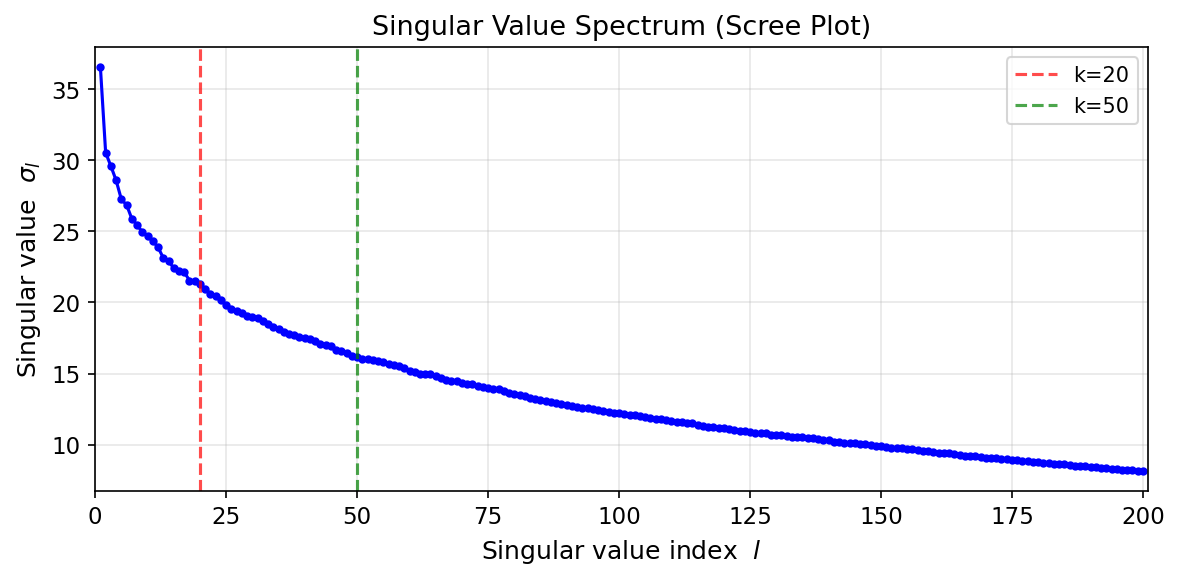
\includegraphics[width=\textwidth]{01_singular_value_decay.png}
      \vspace{0.1em}
      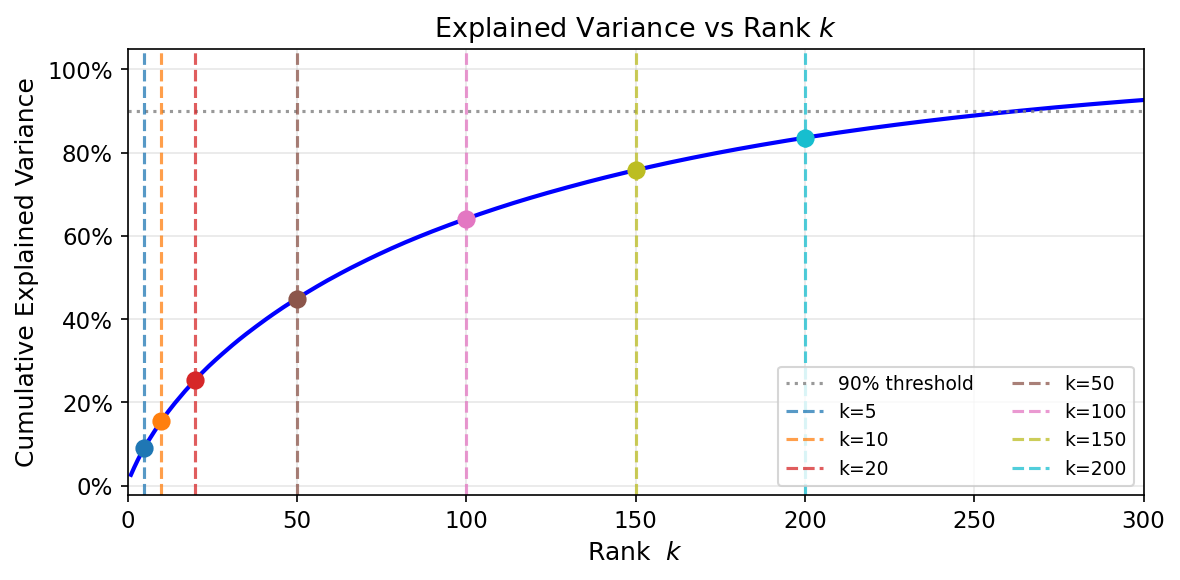
\includegraphics[width=\textwidth]{02_explained_variance.png}
    \end{column}
    \begin{column}{0.46\textwidth}
      \textbf{Key observations:}
      \begin{itemize}
        \item $\sigma_1\approx36.6$,\; $\sigma_{10}\approx24.7$
        \item Ratio $\sigma_1/\sigma_{10}\approx1.48$
        \item Non-flat $\Rightarrow$ \textbf{latent structure}
        \item Flat (Marchenko--Pastur) $\Rightarrow$ pure noise
      \end{itemize}

      \vspace{0.4em}
      \textbf{EV($k$) thresholds:}
      \begin{center}
      \scriptsize
      \begin{tabular}{cr}
        \toprule $k$ & EV($k$) \\ \midrule
        10  & 15.5\% \\
        50  & 44.9\% \\
        100 & 64.1\% \\
        264 & 90.0\% \\
        \bottomrule
      \end{tabular}
      \end{center}

      \vspace{0.2em}
      \small Best RMSE at $k=10$ (EV=15.5\%)\\
      $\ll$ 90\% threshold ($k=264$)
    \end{column}
  \end{columns}
\end{frame}

% ──────────────────────────────────────────────────────────────
\section{Implementation}

\begin{frame}[fragile]{Prediction Formula \& Code Mapping}
  \textbf{Full prediction:}
  \[
    \hat{r}_{ui}
    = \underbrace{\mu+b_u+b_i}_{\text{de-centering}}
    + \underbrace{\sum_{l=1}^k \sigma_l \cdot U_k[u,l]\cdot V_k[i,l]}_{\text{latent interaction}}
  \]

  \textbf{Theory $\leftrightarrow$ Code:}
  \begin{center}
  \scriptsize
  \begin{tabular}{lll}
    \toprule
    \textbf{Equation} & \textbf{Function} & \textbf{File} \\
    \midrule
    $\mu, b_u, b_i$ & \texttt{center\_matrix()} & \texttt{data\_loader.py} \\
    Zero-fill $\tilde{R}$ & \texttt{impute\_matrix()} & \texttt{data\_loader.py} \\
    $R = U\Sigma V^T$ & \texttt{fit\_svd()} & \texttt{svd\_model.py} \\
    $\hat{r}_{ui}$ (batch) & \texttt{predict\_batch()} & \texttt{svd\_model.py} \\
    EY bound & \texttt{eckart\_young\_error()} & \texttt{svd\_model.py} \\
    RMSE, MAE & \texttt{rmse()}, \texttt{mae()} & \texttt{evaluation.py} \\
    \bottomrule
  \end{tabular}
  \end{center}

\begin{lstlisting}
U_scaled = U_k[users] * sigma_k[None, :]    # (N,k): scale user factors
V_cols   = Vt_k[:, items]                    # (k,N): item factors
latent   = np.einsum("nk,kn->n", U_scaled, V_cols)
preds    = np.clip(mu + b_u[users] + b_i[items] + latent, 0.5, 5.0)
\end{lstlisting}
\end{frame}

% ──────────────────────────────────────────────────────────────
\section{Results}

\begin{frame}{Rank Selection: $k$-Sweep Results}
  \begin{columns}
    \begin{column}{0.48\textwidth}
      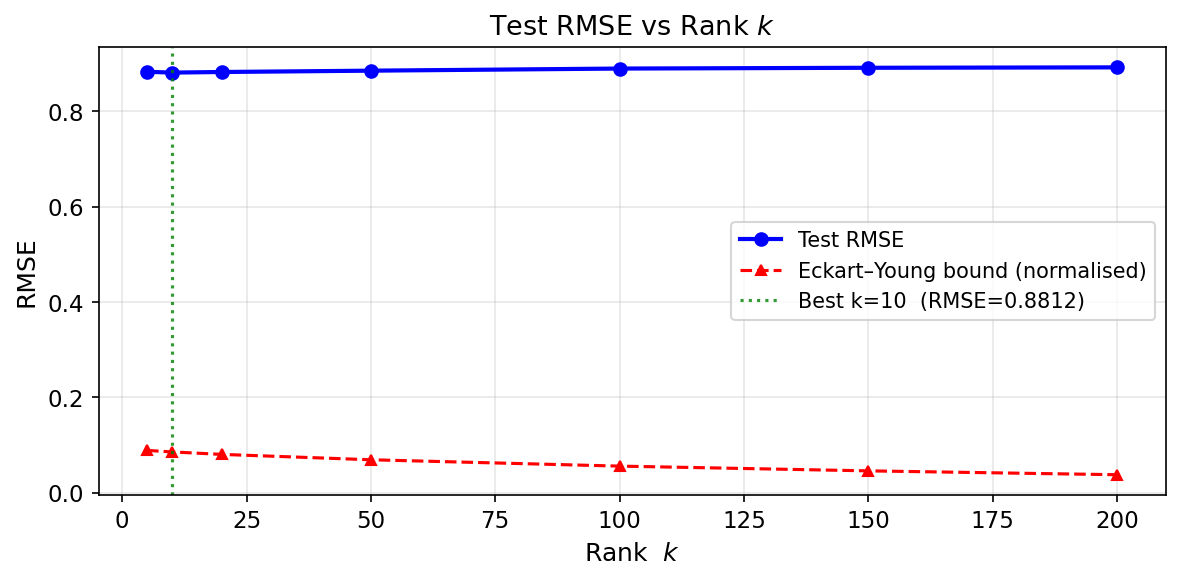
\includegraphics[width=\textwidth]{03_rmse_vs_k.png}
    \end{column}
    \begin{column}{0.48\textwidth}
      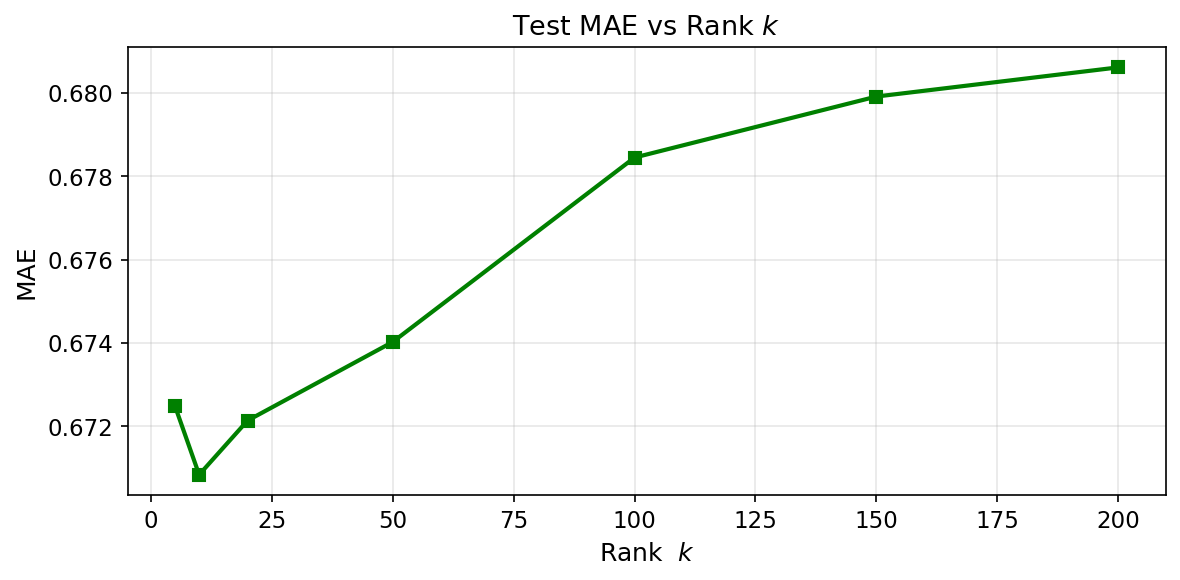
\includegraphics[width=\textwidth]{04_mae_vs_k.png}
    \end{column}
  \end{columns}

  \vspace{0.2em}
  \begin{center}
  \scriptsize
  \begin{tabular}{rrrrl}
    \toprule
    $k$ & RMSE & MAE & EV\% & EY Bound \\
    \midrule
    5   & 0.8829 & 0.6725 &  9\% & 0.760 \\
    \textbf{10}  & \textbf{0.8812} & \textbf{0.6708} & 15.5\% & 0.733 \\
    20  & 0.8825 & 0.6721 & 25\% & 0.688 \\
    50  & 0.8852 & 0.6740 & 45\% & 0.592 \\
    100 & 0.8897 & 0.6784 & 64\% & 0.478 \\
    150 & 0.8913 & 0.6799 & 76\% & 0.392 \\
    200 & 0.8922 & 0.6806 & 84\% & 0.323 \\
    \bottomrule
  \end{tabular}
  \end{center}

  \footnotesize
  $k<10$: underfitting \quad \textbf{$k=10$: optimal} \quad
  $k>10$: overfitting to imputed zeros
\end{frame}

\begin{frame}{Bias--Variance Tradeoff in Rank Selection}
  \begin{columns}
    \begin{column}{0.50\textwidth}
      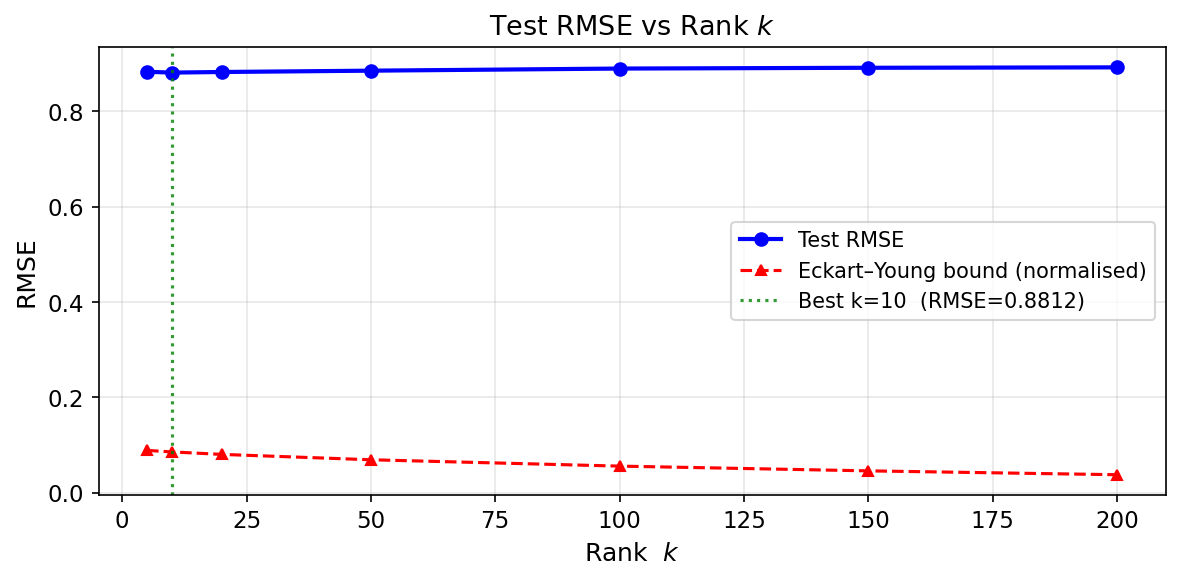
\includegraphics[width=\textwidth]{03_rmse_vs_k.png}
    \end{column}
    \begin{column}{0.48\textwidth}
      \small\textbf{Why does RMSE rise after $k=10$?}
      \begin{itemize}\small
        \item \textbf{Low $k$ (high bias):} too few dimensions to capture
              user-item structure $\Rightarrow$ underfitting
        \item \textbf{High $k$ (high variance):} SVD fits imputed zeros,
              not real ratings $\Rightarrow$ overfitting
      \end{itemize}
      \begin{alertblock}{Key insight: imputation artefact}
        \footnotesize $\min\|\tilde{R}-M\|_F^2 \neq \min\|\mathcal{P}_\Omega(R-M)\|_F^2$\\
        Higher $k$ fits \textbf{zero-fill noise}, not real signal.
      \end{alertblock}
    \end{column}
  \end{columns}
\end{frame}

\begin{frame}{Baseline Model Comparison}
  \begin{columns}
    \begin{column}{0.50\textwidth}
      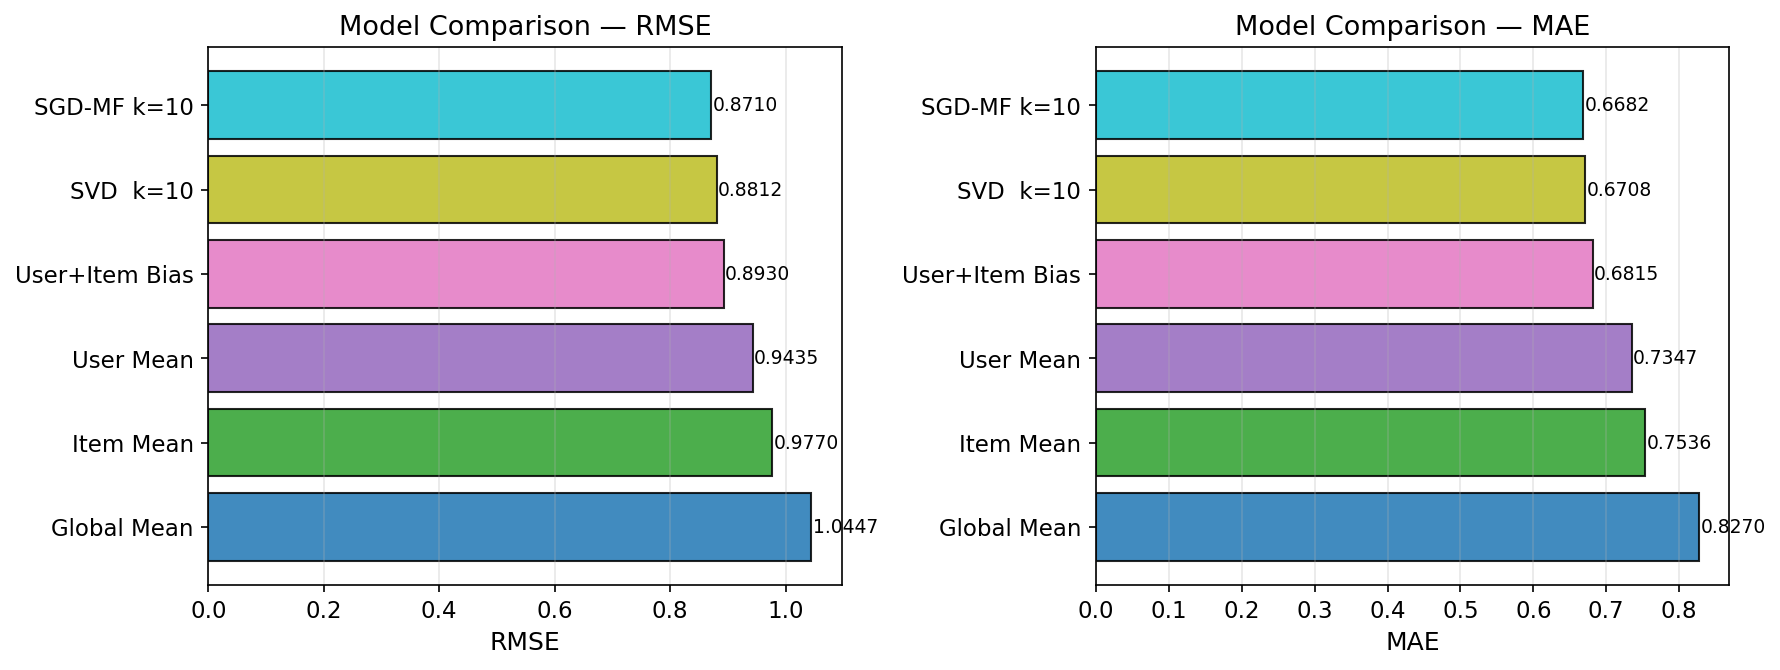
\includegraphics[width=\textwidth]{08_baseline_comparison.png}
    \end{column}
    \begin{column}{0.48\textwidth}
      \small
      \begin{tabular}{lrr}
        \toprule
        \textbf{Model} & \textbf{RMSE} & \textbf{vs Global} \\
        \midrule
        Global Mean      & 1.0447 & --- \\
        Item Mean        & 0.9770 & $-6.5\%$ \\
        User Mean        & 0.9435 & $-9.7\%$ \\
        U+I Bias         & 0.8930 & $-14.6\%$ \\
        \textbf{SVD $k$=10} & \textbf{0.8812} & $\mathbf{-15.6\%}$ \\
        SGD-MF $k$=10    & 0.8710 & $-16.6\%$ \\
        \bottomrule
      \end{tabular}

      \vspace{0.5em}
      \textbf{Key gaps:}
      \begin{itemize}
        \item Bias layers: $-14.6\%$
        \item \textbf{Latent factors (SVD): $-1.3\%$}
        \item Imputation cost: $-1.2\%$
      \end{itemize}
    \end{column}
  \end{columns}
\end{frame}

\begin{frame}{Cross-Dataset Validation: MovieLens 1M}
  \begin{columns}
    \begin{column}{0.54\textwidth}
      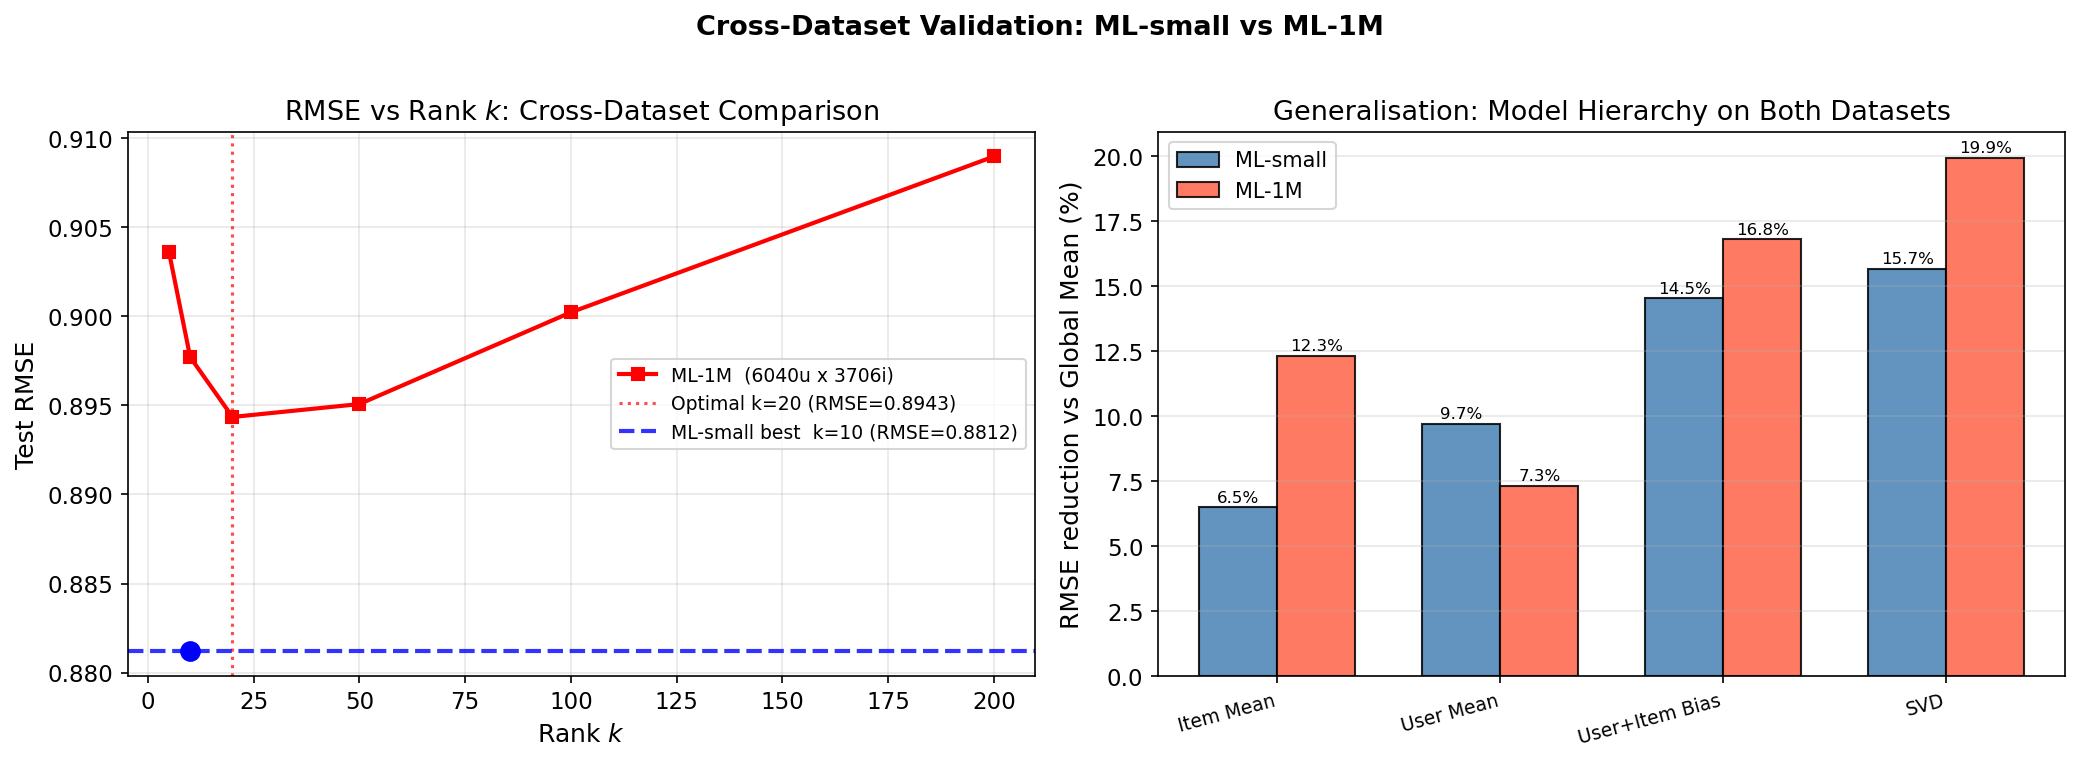
\includegraphics[width=\textwidth]{10_crossdataset_comparison.png}
    \end{column}
    \begin{column}{0.44\textwidth}
      \begin{center}
      \scriptsize
      \begin{tabular}{lcc}
        \toprule
        & \textbf{ML-small} & \textbf{ML-1M} \\
        \midrule
        Users   & 610     & 6,040 \\
        Items   & 9,724   & 3,706 \\
        Ratings & 100,836 & 1,000,209 \\
        Density & 1.36\%  & 4.47\% \\
        \midrule
        Best $k$   & 10     & 20 \\
        RMSE (SVD) & 0.8812 & 0.8943 \\
        MAE  (SVD) & 0.6708 & 0.7021 \\
        \bottomrule
      \end{tabular}
      \end{center}

      \vspace{0.2em}
      \textbf{\small Key findings:}
      \begin{itemize}
        \scriptsize
        \item Model hierarchy preserved on \emph{both} datasets: SVD $>$ U+I Bias $>$ means
        \item Denser ML-1M supports higher $k=20$
        \item \textbf{Methodology generalises} at $10\times$ scale
      \end{itemize}
    \end{column}
  \end{columns}
\end{frame}

\begin{frame}{Latent Factor Interpretation}
  \textbf{Inner-product view:}
  \[
    \hat{r}_{ui} - \mu - b_u - b_i
    = \mathbf{p}_u^\top\,\mathrm{diag}(\boldsymbol{\sigma}_k)\,\mathbf{q}_i
    \quad \mathbf{p}_u,\mathbf{q}_i\in\R^k
  \]

  \begin{columns}
    \begin{column}{0.50\textwidth}
      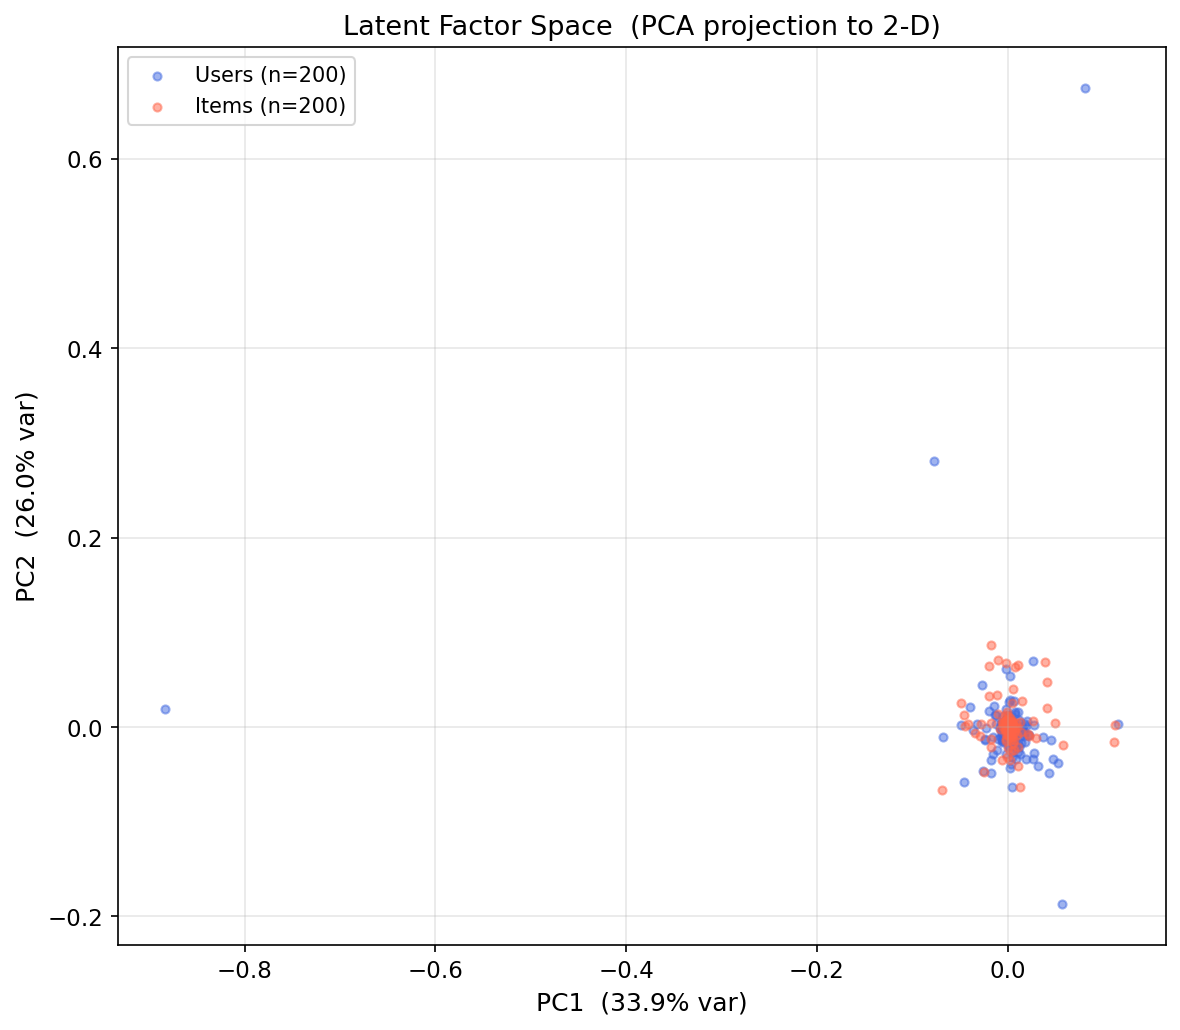
\includegraphics[width=\textwidth]{09_latent_factors.png}
    \end{column}
    \begin{column}{0.48\textwidth}
      \textbf{Geometry:}
      \begin{itemize}
        \item Each user/item: point in $\R^k$
        \item Prediction $\propto$ alignment in latent space
        \item Similar users $\Rightarrow$ nearby points
      \end{itemize}

      \vspace{0.4em}
      \textbf{SVD vs PCA:}
      \begin{itemize}
        \item Both maximise explained variance
        \item SVD: \textbf{jointly optimal}\\
              for users AND items
        \item PCA: one-sided (users only)
      \end{itemize}
    \end{column}
  \end{columns}
\end{frame}

\begin{frame}{SVD vs SGD-MF: Two Solvers, One Problem}
  \begin{columns}[t]
    \begin{column}{0.50\textwidth}
      \begin{block}{SVD (our method)}
        \[
          \min_{\mathrm{rank}(M)\leq k}\FroSq{\tilde{R}-M}
        \]
        \begin{itemize}
          \item Closed-form global optimum (EY)
          \item No extra hyperparameters
          \item $\mathcal{O}(mn\min(m,n))$
        \end{itemize}
      \end{block}
    \end{column}
    \begin{column}{0.48\textwidth}
      \begin{block}{SGD-MF (comparison)}
        \[
          \min_{P,Q,b}\sum_{(u,i)\in\Om}(\cdot)^2 + \lambda\|\cdot\|^2
        \]
        \begin{itemize}
          \item Sparse-aware: no imputation
          \item Local min, iterative
          \item 3 extra hyperparameters
        \end{itemize}
      \end{block}
    \end{column}
  \end{columns}

  \vspace{0.6em}
  \begin{alertblock}{Measured gap ($k=10$)}
    SVD: 0.8812 \quad SGD-MF: 0.8710 \quad
    \textbf{Gap = 0.0102\; (1.2\%)}\\
    \small This gap $=$ exact cost of the zero-imputation approximation
  \end{alertblock}
\end{frame}

% ──────────────────────────────────────────────────────────────
\section{Validation}

\begin{frame}{Rigorous Validation: 48 Tests Passed}
  \begin{center}
  \small
  \begin{tabular}{lrl}
    \toprule
    \textbf{Category} & \textbf{Tests} & \textbf{Key checks} \\
    \midrule
    Data Validation      &  8 & No leakage, NaN semantics, shape \\
    Model Validation     & 12 & EY property, orthonormality, bounds \\
    Metrics Validation   &  9 & Manual RMSE/MAE, Jensen's inequality \\
    Bias Decomposition   &  4 & Zero mean, exact reconstruction \\
    Reproducibility      &  4 & Seed 42, SVD determinism \\
    Edge Cases           &  5 & Cold-start, sparse rows \\
    Performance          &  3 & SVD $<$5s, SGD $<$30s \\
    Results Consistency  &  3 & Sorted table, valid RMSE range \\
    \midrule
    \textbf{Total} & \textbf{48} & \textbf{All passed in 1.39s} \\
    \bottomrule
  \end{tabular}
  \end{center}

  \textbf{Critical tests:}
  \begin{itemize}
    \item \texttt{test\_eckart\_young}: $\|A-A_k\|_F^2 = \sum_{l>k}\sigma_l^2$ to $10^{-8}$
    \item \texttt{test\_train\_test\_no\_leakage}: zero (userId, movieId) overlap
    \item \texttt{test\_batch\_vs\_scalar}: \texttt{predict()} $\equiv$ \texttt{predict\_batch()} to $10^{-10}$
  \end{itemize}
\end{frame}

% ──────────────────────────────────────────────────────────────
\section{Conclusions}

\begin{frame}{Summary, Limitations \& Future Work}
  \begin{columns}[t]
    \begin{column}{0.50\textwidth}
      \textbf{Summary:}
      \begin{itemize}
        \item Formal $\min\|\cdot\|_F^2 \to$ Eckart--Young (optimal)
        \item SVD $k=10$: RMSE $= 0.8812$ (ML-small)
        \item $-15.6\%$ vs global; $-1.3\%$ vs bias
        \item 48/48 tests $\mid$ 7-point $k$-sweep
        \item \textbf{Cross-dataset:} generalises to ML-1M\\
              ($10\times$ scale; RMSE $= 0.8943$, $k=20$)
      \end{itemize}

      \vspace{0.4em}
      \textbf{Limitations:}
      \begin{enumerate}
        \small
        \item Linearity (no interaction terms)
        \item Cold start (no new-user embed)
        \item Imputation bias ($+1.2\%$ vs SGD-MF)
        \item Static (no temporal drift)
        \item Scalability $\mathcal{O}(mn\min(m,n))$
      \end{enumerate}
    \end{column}
    \begin{column}{0.48\textwidth}
      \textbf{Future directions:}
      \begin{itemize}
        \item \textbf{Randomised SVD} (Halko 2011)
        \item \textbf{Temporal SVD++} (Koren 2010)
        \item \textbf{Neural CF} (He 2017)
        \item \textbf{ALS / WALS} (sparse-aware)
      \end{itemize}

      \vspace{0.6em}
      \begin{block}{}
        \centering
        \textbf{Thank you.}\\
        \small Questions welcome.
      \end{block}
    \end{column}
  \end{columns}
\end{frame}

% ──────────────────────────────────────────────────────────────
\appendix

\begin{frame}{Appendix A: Eckart--Young Proof Sketch}
  \textbf{Claim:} $A_k$ minimises $\FroSq{A-B}$ over all rank-$k$ matrices $B$.

  \textbf{Proof sketch:}
  \begin{enumerate}
    \item \textbf{Frobenius--spectral identity:}\;
          $\FroSq{A} = \sum_l\sigma_l^2$
    \item For any rank-$k$ matrix $B$, by von Neumann's trace inequality:
          $\;\langle A,B\rangle_F \leq \sum_{l=1}^k\sigma_l(A)\sigma_l(B)$
    \item Substituting into $\FroSq{A-B}=\FroSq{A}-2\langle A,B\rangle_F+\FroSq{B}$:
          \[
            \FroSq{A-B} \;\geq\; \sum_{l=k+1}^r\sigma_l^2
          \]
    \item Equality at $B = A_k$:\;
          $\FroSq{A-A_k} = \sum_{l=k+1}^r\sigma_l^2$ \checkmark
  \end{enumerate}

  Top-$k$ singular vectors form the \textbf{optimal} $k$-dimensional column subspace
  (minimax characterisation of singular values).

  \vspace{0.3em}
  \textbf{Code verification:}
  \texttt{test\_eckart\_young\_reconstruction} confirms to $10^{-8}$ precision.
\end{frame}

\begin{frame}{Appendix B: Evaluation Protocol}
  \textbf{Protocol:}
  \begin{enumerate}
    \item Stratified 80/20 split by user (every user in both splits)
    \item Matrix built from training ratings only (\textbf{zero leakage})
    \item Full vocabulary: test users/items always indexable
    \item Cold-start entries silently skipped in evaluation
    \item Metrics on $N = 19{,}940$ test ratings
  \end{enumerate}

  \[
    \text{RMSE} = \sqrt{\frac{1}{|T|}\sum_{(u,i)\in T}(r_{ui}-\hat{r}_{ui})^2},
    \qquad
    \text{MAE} = \frac{1}{|T|}\sum_{(u,i)\in T}|r_{ui}-\hat{r}_{ui}|
  \]

  \textbf{Why both?}
  \begin{itemize}
    \item RMSE: quadratic penalty on outliers; MAE: linear, robust
    \item RMSE $\geq$ MAE always (Jensen's inequality on $\sqrt{\cdot}$)
    \item Both select $k=10$ as optimal $\Rightarrow$ result is robust to metric choice
  \end{itemize}

  \textbf{Reproducibility:} Seed 42.
  \texttt{test\_same\_seed\_same\_split} and \texttt{test\_svd\_deterministic}
  confirm identical results across independent runs.
\end{frame}

\end{document}
